
\documentclass[12pt,a4paper,twoside]{article}

\usepackage[utf8]{inputenc}
\usepackage[ngerman]{babel}
\usepackage{amsmath,amssymb,amsfonts}
\usepackage{todonotes}
\usepackage{algorithm}
\usepackage{listings}
\usepackage{algpseudocode}
\begin{document}

\lstset{
basicstyle=\small\ttfamily,
xleftmargin=3.5em,
language=Promela,
captionpos=b
}

\title{Text classification mit Machine Learning Methoden}
\author{Lukas Hofmaier \texttt{lukas.hofmaier@hsr.ch}}
\maketitle

\section{Das Text Classification Problem}
\label{sec:problem}

Dieser Abschnitt gibt erkl"art, worum es bei Text Classication geht.

Es gibt folgende Ansatze um eine Menge von Dokumenten in Klassen zu unterteilen:
\begin{description}
\item[Manuelle Klassifizierung] Eine Person ordnet Text manuell einem bestimmten Thema zu. Dieser Ansatz skaliert nicht.
\item[Standing queries] Es werden f"ur jedes Thema eigene Queries geschrieben, die in einer Menge von Dokumenten die richtigen finden. Dieser Ansatz funktioniert sehr gut. Die Regeln m"ussen f"ur jedes Thema einzeln angefertigt werden. Gute Regeln erfodern, dass der Autor der Regel sich mit Queries und der Domain auskennt.
\item[Machine learning-based] Der Computer generiert eine Regel aufgrund von richtigen Zuordnungen. Diese Regel kann danach auf neue Dokumente angewandt werden.
\end{description}


Bei Text Classification geht es darum, Dokumente vordefinierten Klassen zuzuordnen. Man m"ochte eine Menge von Dokumenten in Klassen unterteilen. Sucht man nur nach Dokumenten einer bestimmten Klasse, muss man nicht jedes Dokument manuell "uberpr"ufen, ob es relevant ist. Klassen k"onnen z.B. Themen sein. Man k"onnte die Dokumente zu einem Thema suchen, indem man einen boolschen Ausdruck definiert, der ausdr"uckt welche W"orter in einem Dokument enthalten sein m"ussen. Dieser Ansatz hat den Nachteil, dass es schwierig ist, geeignete boolsche Ausdr"ucke zu formulieren, die zu guten Resultaten f"uhren.

Eine anderer Ansatz ist machine learning-based Text Classification. Bei diesem Ansatz wird die Regel nach, der man Dokumente, den Klassen zuteilt, aus sogenannten Trainings Daten, berechnet. Die Trainingsdaten (training set $\mathbb{D}$ ) bestehen aus einer Menge von Dokumenten, denen bereits die richtige Klasse zugeordnet wurde. Diese Zuordnung kann z.B. manuell passieren. Dieser Ansatz wird auch supervised learning oder "uberwachtes Lernen genannt. 

Die generierte Regel, wird auch Klassifizierer oder Entscheidungsfunktion $\gamma$ genannt.
\[
\gamma : \mathbb{X} \to \mathbb{C}
\]

$\mathbb{X}$ ist der Document space und $\mathbb{C}$ ist die Menge aller Klassen. Der Klassifizierer nimmt ein Dokument als Input und gibt die passende Klasse zur"uck. F"ur Dokumente gibt es unterschiedliche Repr"asentationen. Eine m"ogliche Repr"asentation wird in Abschnitt \ref{sec:vectorspacemodel} erkl"art.

Die Trainingsdaten sind der Input der Lernmethode $\Gamma$. $\Gamma$ gibt die Entscheidungsregel $\gamma$ zur"uck.
\[
\Gamma(\mathbb{D}) = \gamma
\]

\section{Dokumenterepr"asentation}
\label{sec:linearclassifiers}

\subsection{Vector space model}
\label{sec:vectorspacemodel}
Die Klassifizierungsfunktion $\gamma$ bestimmt f"ur ein gegebenes Dokument $d$ die Klasse $c$. Bei den folgenden Klassifizierer muss das Dokument als Vektor re\-pr"as\-entiert werden. Der folgenden Abschnitt beschreibt die Repr"asentation eines Dokumentes als Vektor.

\subsubsection{TF-IDF}
\label{sec:tfidf}

Um Dokumente mit den nachfolgenden Methoden zu klassifizieren, wird jedes Dokument als Vektor gespeichert. Jedem Wort von Interesse wird ein Wert zugeordnet. Eine einfache M"oglichkeit, w"are die Anzahl des Auftretens f"ur jedes Wort in dem Vektor abzuspeichern. Diese Repr"asentation ber"ucksichtig nicht, dass allgemeine W"orter wie z.B. Auto, wenig "uber den Inhalt eines Dokumentes aussagen, aber trotzdem, oft vorkommen.

Um die Seltenheit eines Wortes zu bestimmen, wird die Anzahl der Dokumente, die das Wort enthalten bestimmt. Wenn $N$ die Anzahl aller Dokumente ist, kann mit der Formel

\[
idf_t = log \frac{ N}{df_f}
\]

die Seltenheit des Wortes bestimmt werden. Der Wert $idf_t$ zu einem Wort $t$ ist umso h"oher umso seltener ein Wort in einer Menge von Dokumenten vorkommnt. Man nennt diesen Wert inverse document frequency\cite{manning08}.

Die Anzahl des Auftretens eines Wortes $t$ innerhalb eines Dokumentes $d$ wird term frequency $tf_{t,d}$ genannt.

Die Werte $tf$ und $idf$ werden zu dem sogenannten $tf-idf$ Wert kombiniert. Dieser berechnet sich f"ur ein Wort $t$ in einem Dokument $d$ wie folgt:
\[
tf-idf_{t,d} = tf_{t,d} \times idf_t
\]

% \begin{table}
%   \centering
%   \begin{tabular}{l l l l l l}
%     & Dok1 & Dok2 & Dok3 & idf & tf-idf Dok1 \\
%     Chip & 27 & 4 & 24 & 1.65 &44.5  \\
%   \end{tabular}
%   \caption{tf-idf Beispiel Werte }
%   \label{tab:temporal_operators}
% \end{table}

\todo{Tabelle mit m"oglichen idf tf tf-idf werten einfuegen}

Bei Text classication geht es darum, "ahnliche Dokumente zu finden. Jedem Wort in einem Dokument kann der $tf-idf$ - Wert zugewiesen werden, dass heisst jedes Dokument kann als Vektor, dessen Komponenten $tf-idf$ Werte sind repr"asentiert werden. Werden alle Dokumente, die klassifiert werden, als tf-idf-Vektoren mit einem gemeinsamen Vektorraum dargestellt, spricht man vom vector space model.

\subsection{Vector space classification}
\label{sec:vectorclassification}

Wie in Abschnitt \ref{sec:vectorspacemodel} erk"art, k"onnen Dokumente als Vektoren dargestellt werden. Um die Funktionsweise der nachfolgenden Methoden zu erkl"aren, haben diese Vektoren zwei Komponente. Wenn es dabei um Vektoren mit zwei Komponenten handelt, k"onnen diese als Punkte in der Ebene dargestellt werden. In der Realit"at arbeitet man mit Vektoren die Punkte in einer Hyperebene darstellen.

Wenn alle Dokumente als Punkte in der Ebene dargestellt werden, de\-finiert ein linearer Klassifizierer eine Linie in dieser Ebene. Ein Algorithmus, der neue Dokumente klassifiziert, muss entscheiden, ob die Vektor space Repr"a\-sentation des Dokuments auf welcher Seite liegt. Die Linie wird auch decision boundary genannt. Die Herausforderung der text classification liegt darin, gute decision boundaries zu finden.

\todo{Bild von 2D Plane mit decision boundiary erstellen}

\section{Logistische Regression}
\label{sec:logisticreg}

Ein Klassifizierer kann ein neues Objekt, das als Vektor repr"asentiert wird, einer Klasse zuteilen. In nachfolgenden Abschnitt geht es immer darum ein Objekt in eine von zwei Klassen einzuteilen. Den Klassen k"onnen mit den Zahlen 1 und 0 beschriftet (gelabelt) werden. Ein Klassifizierer nimmt als Input einen Vektor und gibt 0 oder 1 aus. Ein solcher Klassifizierer kann als Funktion modelliert werden, die 0 oder 1 ausgibt. Da eine Funktion, die nur die beiden diskreten Werte 0 oder 1 ausgibt, mathematisch schwieriger zu handhaben ist, nutzt man die sogenannnte Sigmoidfunktion. Abbildung \ref{fig:sigmoidfunc} zeigt einen Plot der Sigmoidfuncktion. 

\[
g(z) = \frac{1}{1 + e^{-z}}
\]


\begin{figure}
  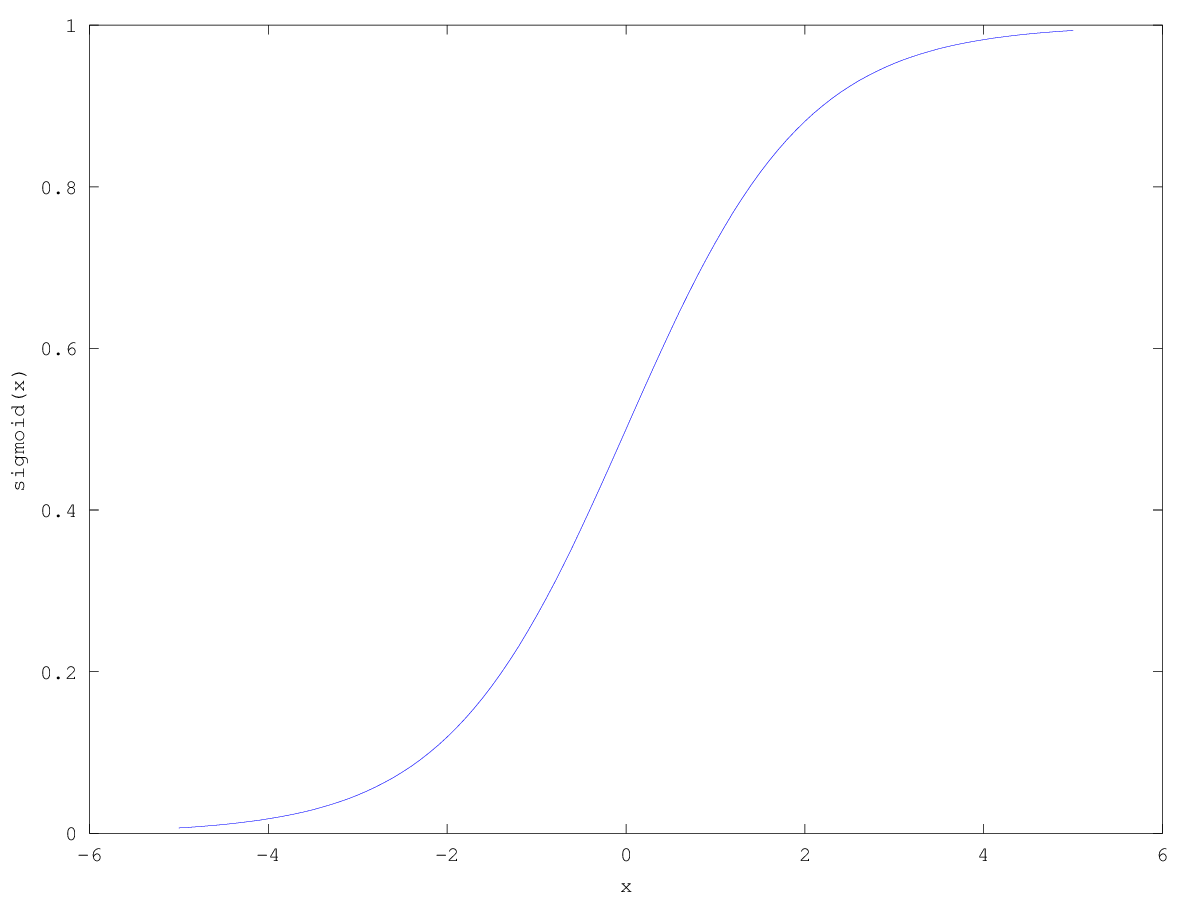
\includegraphics[scale=0.3]{sigmoid}
  \centering
  \label{fig:sigmoidfunc}
  \caption{Plot der Sigmoidfunktion}
\end{figure}

Der Wertebereich der Sigmoidfunktion liegt zwischen 0 und 1. Bei einer Eingabe von 0 gibt die Funktion 0.5 zur"uck.

Der Klassifizierer berechnet das Skalarprodukt des Featurevektor $x$ und einem Paramatervektor $\Theta$ Theta aus.

\[
z = \Theta^T x
\]

Dieser Wert dient als Input f"ur die Sigmoidfunktion. Ist der Wert gr"osser 0.5, das heisst das Skalarprodukt ist gr"osser 0, wird das Objekt der Klasse mit dem Label 1 zugewiesen. Ist der Wert kleiner 0.5 wird das Objekt der Klasse mit Label 0 zugewiesen. Die Aufgabe des Klassifizierungalgorithmus ist es, die Werte des Parametervektors zu bestimmen, so dass m"oglichst viele Objekte in den Trainingsdaten richtig klassifiziert werden. 

\subsection{Kostenfunktion}
\label{sec:costfunction}

Der Klassifizierer soll denjenigen Paramtervektor $\Theta$ finden, der die Objekte der Trainingsmenge mit der gr"ossten Wahrscheinlichkeit richtig einordnen kann. Um zu bestimmen wie gut die Wahl der Koeffizienten $\Theta$ ist, wird folgende Funktoin verwendet.

\begin{equation}
  \label{eq:costfunction}
  J(\theta) = \left \{
    \begin{array}{l l}
      -\log(h_{\theta} (x)) & \quad \text{if $y==1$}\\
      -\log(1-h_{\theta} (x)) & \quad \text{if $y==0$}
    \end{array} \right.
\end{equation}

Diese Funktion \ref{eq:costfunction} gibt f"ur $y==1$ grosse Werte zur"uck, wenn $h_{\theta}$ nahe bei $0$ liegt und sie gibt genau $0$ zur"uck, wenn $h_{\theta}$ $1$ ist. Das heisst, wenn $h_{\theta}$ und $y$ "ubereinstimmen ist der Wert klein, sonst gross. Bei $y==0$ ist es genau umgekehrt. Und der Klassifiziereralgorithmus soll $\theta$ so w"ahlen, dass $h_{\theta}$ und $y$  f"ur alle Trainingsbeispiele m"oglichst "ubereinstimmen. Die Funktion \ref{eq:costfunction} soll also minimiert werden.

\begin{equation}
  \label{eq:minimize}
  \underset{\theta}{\text{min}} J(\theta)
\end{equation}

Diese Funktion kann ohne Unterscheidung, ob $y$ 1 oder 0 ist, wie folgt geschrieben werden. 

\begin{equation}
  \label{eq:simplecostfunction}
  J( \theta ) = - \frac{1}{m} \sum_{i=1}^m y^{(i)} \log h_{\theta}(x^{(i)}) + (1 - y^{(i)}) \log(1 - h_{\theta}(x^{(i)}))
\end{equation}

Die Kostenfunktion z"ahlt die Abweichungen vom Sollwert aller $m$ Trainingsbeispiele zusammen. $x^{(i)}$ und $y^{(i)}$ bezeichnen ein Objekt aus der Trainingsmenge.

Die Funktion $J(\theta)$ gibt kleine Werte zur"uck, wenn $\theta x$ Werte sind, die weiter entfernt von 0 sind. Das heisst, je weiter weg die Objekte der Trainingsmenge von der descision boundary. Der Klassifizierer soll eine Descision Boundary finden, die von allen Punkten den gr"ostm"oglichen Abstand hat. Die Funktion $J(\theta)$ soll also minimiert werden. Dies kann beispielsweise mit dem Gradientenabstieg gemacht 

\subsection{Gradientenverfahren}
\label{sec:gradientdescent}

Im Abschnitt \ref{sec:costfunction} haben wir gezeigt, dass die Decision Boundary f"ur einen Klassifizierer algorithmisch gefunden werden kann, indem die Kostenfunktion \ref{eq:simplecostfunction} minimiert wird. Der Algorithmus soll die Paramter $\theta$ finden, so dass \ref{eq:simplecostfunction} minimiert wird. Eine M"oglichkeit die Kostenfunktion zu minimeren ist das Gradientenverfahren. Der Gradient einer Funktion zeigt in die Richtung des steilsten Aufstiegs \cite{teschl07}. Der negative Gradient in Richtung des steilsten Abstiegs. Wenn man den negativen Gradienten von der aktuellen Position subtrahiert, wird die Funktion ein wenig minimiert. Wiederholt man diesen Schritt beliebig oft, konvergiert der Algorithmus irgendwann bei einem lokalen Minimum. Wie gross die Schritte in Richtung Minimum sind, wird mit dem Paramter $\alpha$ festgelegt. Der Gradient ist ein Vektor dessen Elemente die partiellen Ableitungen jedes einzelnen Features sind.

\begin{algorithm}
\caption{Gradientenverfahren}
\begin{algorithmic}

\Repeat \{ \\
$\theta_j := \theta_j - \alpha \frac{\partial}{\partial \theta_j} J(\theta)$  \\
\}
\Until $\theta$ konvergiert 

 \end{algorithmic}  
\end{algorithm}

Wir wenden das Gradientenverfahren auf die Kostenfunktion an. Zuerst wird die Kostenfunktion partiell abgeleitet.
\begin{equation}
  \label{eq:costderivativ}
  \frac{\partial}{\partial \theta_j} J(\theta) = \frac{1}{m} \sum_{i=1}^m (h_{\theta} (x^{(i)}) - y^{(i)})x_j^{(i)}
\end{equation}

Die abgeleitete Kostenfunktion kann man im Gradientenverfahren einsetzen und erh"alt:
\begin{algorithm}
\caption{Gradientenverfahren}
\begin{algorithmic}

\Repeat \{ \\
$\theta_j := \theta_j - \alpha \frac{\partial}{\partial \theta_j} J(\theta) = \frac{1}{m} \sum_{i=1}^m (h_{\theta} (x^{(i)}) - y^{(i)})x_j^{(i)}$  \\
\}
\Until $\theta$ konvergiert 

 \end{algorithmic}  
\end{algorithm}

Das Gradientenverfahren liefert den Vektor $theta$ der ein Minimum der Kostenfunktion findet. Mit diesem $\theta$ k"onnen neue Instanzen nach der folgenden Regel klassifiziert werden.

Wenn $\theta^T x \geq 0$ dann $y=1$

Wenn $\theta^T x < 0$ dann $y=0$

Das Listing \ref{lst:logisticregression} zeigt eine Implementation in Octave des Verfahrens.

\subsection{Implementation}
\label{sec:implementation}
Die Trainingsbeispiele werden in eine Matrix geladen. In dieser Matrix entspricht jede Zeile einem Objekt. Die korrekte Klassifizierung wird in einen Vektor y geladen. Die Elemente von y sind 1 oder 0. In der Variablen \verb|m| wird die Anzahl der Beispiele gespeichert. In der Beispielimplementation werden die Objekte mit zwei reelen Zahlen beschrieben. Dass heisst die Matrix \verb|X| hat die Dimension $m \times 2$. Um die Hypthesenfunktion einfach auf alle Beispiele anzuwenden, wird der Matrix \verb|X| eine Kolonne mit 1en hinzugef"ugt. Dadurch kann man mit der Matrix-Vektor Multiplikation von allen Beispielen den Wert der Hypthesenfunktion ausrechnen.

\begin{lstlisting}
h_theta = sigmoid(X * theta);
\end{lstlisting}

Der Gradient der Kostenfunktion berechnet sich wie folgt:

\begin{equation}
\frac{1}{m} \sum_{i=1}^m (h_{\theta} (x^{(i)}) - y^{(i)})x_j^{(i)}  
\end{equation}

Die Berechnung dieses Term k"onnte man mit einem for-loop "uber alle Beispiele der Trainingsmenge implementieren. Eleganter und einfacher auf mehrere Cores zu verteilen ist folgenden Implementation:

\begin{lstlisting}
function grad = gradient(theta, X, y)
m = length(y);
h_theta = sigmoid(X * theta);
grad = 1/m .* (X' * (h_theta - y));
end
\end{lstlisting}

Der Ausdruck 
\begin{lstlisting}
X' * (h_theta - y)
\end{lstlisting}
summiert alle Produkte $(h_{\theta} (x^{(i)}) - y^{(i)})x_j^{(i)}  $ "uber die gesamte Trainingsmenge. Somit wird

\begin{equation}
   \sum_{i=1}^m (h_{\theta} (x^{(i)}) - y^{(i)})x_j^{(i)}
\end{equation}

berechnet.

\subsection{Regularisation}
\label{sec:regularization}

Um Overfitting zu vermeiden, begrenzt man die Werte in $\theta$. Dies wird dadruch erreicht, dass man der Kostenfunktion den Term $\frac{\lambda}{2m} \sum_{j=1}^n \theta^2$ hinzuf"ugt. Es wird also foglende Funktion minimiert.
\begin{equation}
  \label{eq:regularization}
  \underset{\theta}{\text{min}}  J(\theta) = -\frac{1}{m} \sum_{i=1}^m y^{(i)} \log h_{\theta}(x^{(i)}) + (1 - y^{(i)}) \log(1 - h_{\theta}(x^{(i)}))+\frac{\lambda}{2m} \sum_{j=1}^n \theta^2
\end{equation}

\section{Support vector machines}
\label{sec:svm}

Dieser Abschnitt beschreibt einen weiteren Klassifikationsalgorithmus. Es geht um Support Vector Machines (SVM's). Dieser Algorithmus ist in der Industrie sehr verbreitet.

Bei logistischer Regression soll sich die Hypothesenfunktion $h_{\theta}$ wie folgt verhalten.
Wenn $y == 1$, dann soll $h_{\theta} \approx 1$, Dass heisst $\theta^T x \gg 0$. Und wenn $y == 0$, dann $h_{\theta} \approx 0$. Bei SVM wird gefordert, dass $\theta^T x \geq 1$ f"ur $y == 1$ und $\theta^T x \leq -1$ f"ur $y == 0$.

Wenn $\theta$ diese Beschr"ankung einh"alt, tr"agen die Objekte in der Trainimgsmenge nichts zu Kostenfunktion bei.

Der erste Teil der Optimierungsproblems der logistischen Regression
\begin{equation}
  \label{eq:costsvm}
\underset{\theta}{\text{min}}   = y^{(i)} cost_1(h_{\theta}(x^{(i)})) + (1 - y^{(i)})(cost_2(h_{\theta}(x^{(i)}))) 
\end{equation}
wird 0. Dass heisst es bleibt nur noch

\begin{equation}
  \label{eq:opt}
  \underset{\theta}{\text{min}}  J(\theta) = \frac{\lambda}{2m} \sum_{j=1}^n \theta^2
\end{equation}

Man nennt SVM's auch Large Margin Classifier weil die decision boundary so

Wie in Abschnitt \ref{sec:vectorclassification} erkl"art, definiert ein Klassifizierer eine Hyperebene. Diese ist definiert durch den Achsenabschnitt $b$ und den Normalenvektor $ \vec w $. Alle Punkte $\vec x $ die auf dieser Hyperebene liegen, erf"ullen die Gleichung 
\[
\vec w^T \vec x = -b
\].

Neue Dokumente k"onnen wie folgt klassifiziert werden: Die Funktion
\[
f(\vec x ) = sign( \vec w^T \vec x + b)
\]
wird ausgewertet. Je nachdem, ob der Wert $1$ oder $-1$ ist wird das Dokument einer Klasse zugeordnet.

Support Vectors (St"utzvektoren) sind die Objekte die am nahesten bei der Decision Boundary sind. SVM's finden eine Hyperebene, die die Datenmenge so trennt, dass die St"utzvektoren m"oglichst weit entfernt von der Decision Boundary sind. Der Abstand von Punkten die der Decision Boundary am n"achsten sind, soll also  maximiert werden. Man sagt dazu, dass die Daten mit maximaler Trennspanne getrennt werden $\vec w$ muss folgende Forderung erf"ullen.

\[
\vec w^T \vec x_i + b \geq 1 \text{f"ur} y_i = 1
\]

\[
\vec w^T \vec x_i + b \leq 1 \text{f"ur} y_i = 0
\]

Der Abstand von einem Punkt zur Hyperebene l"asst sich berechnen durch

\[
\frac{\vec w}{||w||} \vec x_i + \frac{b}{||w||}
\]

Das heisst die beiden Punkte, die der Decision Boundary am n"achsten sind, haben jeweils den Abstand $\frac{1}{||w||}$. Die gesamte Trennspanne ist also $\frac{1}{||w||}$. Die Trennspanne soll maximiert werden. Das heisst $||w||$ soll minimiert werden. Um die beste Decision Boundary zu finden m"ussen wir folgendes Optimierungsproblem l"osen.

 \begin{equation*}
\begin{aligned}
& \underset{x}{\text{minimiere}}
& & \lVert \vec w \rVert^2 \\
& \text{subject to}\\
& & \vec{w}^T \vec{x_i} + b \geq 1, \; y_i = 1 \\
& & \vec{w}^T \vec{x_i} + b \leq -1, \;  y_i = 0
\end{aligned}
\end{equation*}

Das ist ein Optimierungsproblem mit Nebenbedingung. Es kann in eine Lagrangefunktion zusammengefasst werden \cite{cristianini}. Wenn man die Lagrangefunktion ensprechend umformt erh"alt man folgendes Optimierungsproblem. Die Funktion

\begin{equation}
  \label{eq:dualrep}
W(\alpha) = \sum_{i=1}^n \alpha_i - \frac{1}{2} \sum_{i,j = 1}^n \alpha_i \alpha_j y_i y_j \vec{x_i^T} \vec{x_j}  
\end{equation}

soll unter der Bedingung
 \[
\alpha_i \geq 0
\sum_{i=0}^n \alpha_i y_i = 0
\]

Die Umformung ist wichtig, weil in \ref{eq:dualrep} das Skalarprodukt von zwei Featurevektoren ausgerechnet wird. Das kann man ausnutzen.

\subsection{Klassifizieren von nichtlinearen Daten}
\label{sec:nonlinear}

Die Decisionboundary, die man erh"alt, wenn man \ref{eq:dualrep} l"ost, ist eine Hyperebene. Im 2D Raum ist das eine Linie. Im 3D-Raum eine Ebene. Damit k"onnen nur linear separierbare Objekte klassifiziert werden. Es ist jedoch m"oglich die Daten der Objekte so zu transformieren, dass neue Dimensionen dazu kommen. Den neuen Vektorraum nennt man Feature Space. Ein zweidimensionaler Vektor kann zum Beispiel wie folgt transformiert werden.

\begin{equation}
  \label{eq:polynomial}
\Phi: (x_1, x_2) \mapsto (x_1^2, \sqrt{2} x_1 x_2, x_2^2)
\end{equation}

Die Abbildung $\Phi$ f"ugt dem Input Space eine zus"atzliche Dimension hinzu. Im Feature sind die Daten unter Umst"anden linear trennbar und k"onnen deshalb mit jedem Algorithmus f"ur lineare Klassifikation klassifiziert werden. Dieser Ansatz funktioniert auch beim Algorithmus f"ur logistische Regression. Das Mapping vom Input space muss f"ur jedes Objekt durchgef"uhrt werden und skaliert dementsprechend schlecht. 

Im Featurespace m"ussen Skalarprodukte der Form $\Phi(\vec{x_i})^T \Phi(\vec{x_j})$ ausgerechnet werden (siehe Gleichung \ref{eq:dualrep}). Dieses Skalarprodukt kann mit einer sogenannten Kernel-Funktion $\mathcal{K}$ ausrechnet werden. Der Wert von $\mathcal{K}$ ist im Inputspace gleich dem Skalarprodukt der beiden Operatoren im Featurespace.
\begin{equation}
  \label{eq:kerneltrick}
  \mathcal{K}(x_i, x_j) = \Phi(x_i)^T \Phi(x_j)
\end{equation}

Es kann gezeigt werden, dass nach Umformen des Skalarprodukt der Featurevektoren, die mit $\Phi$ berechnet wurden, gleich dem Wert von $\mathcal{K}$ ist im urspr"unglichen Inputspace ist.

\begin{eqnarray}{lcl}
  \label{eq:transformkernel}
  \Phi((x_1, x_2)) \cdot \Phi((y_1, y_2)) & = & (x_1^2, \sqrt{2} x_1 x_2, x_2^2)(y_1^2, \sqrt{2} y_1 y_2, y_2^2)\\
& = & x_1^2 y_1^2 + 2 x_1 x_2 y_1 y_2 + x_2^2 y_2^2 \\
& = & (x_1 y_1 + x_2 y_2)^2 \\
& = & \vec{x}^T \vec{y} \\
& = & \mathcal{K}
\end{eqnarray}

Es ist also gar nicht n"otig die Funktion $\Phi$ anzuwenden. Wenn das Skalarprodukt eine Kernelfunktion ist m"ussen wir die $\vec{w}$ nicht in einem hochdimensionalen Raum berechnen. Das spart viel Rechen und Speicheraufwand. Man nennt diese Abk"urzung den Kerneltrick. Weil SVM's das Skalarprodukt in der Gleichung \ref{eq:dualrep} enthalten, kann der Kernel Trick bei SVM angewendet werden. Das verringert die Laufzeit.

\appendix

\section{Octave Demo: Logistische Regression}
\label{sec:code}


\section{Rocchio classification}
\label{sec:rocchio}

Rocchio classifiation ist ein m"ogliches Verfahren um Dokumente zu klassifizieren. Die Grenzen zwischen den Klassen werden mit sogenannten centroids definiert. Ein centroid ist eine Vektor, dessen Komponente die Durchschnitts\-werte aller Vektoren der selben Klasse darstellen.
\[
\vec \mu(c) = \frac{1}{|D_c|} \sum_{d \in D} \vec v (d)
\]
$\vec (d)$ ist die Vektor space Repr"asentation. $D_c$ ist die Menge aller Dokumente der Klasse, dessen centroid berechnet werden soll.

Neue Dokumente werden nach folgender Regel zugeordnet: Es wird die tdf-idf repr"asentation $\vec v (d)$ f"ur das neue Dokument $d$ berechnet. Dann wird $d$ derjenigen Klasse zugeordnet zu dessen centroid $\vec v (d)$ die geringste Distanz hat.

\begin{algorithm}
\caption{Rocchio Trainings-Algorithmus}
\begin{algorithmic}

\ForAll{ $c_i \in $ Klasses} 
\State $ D_j \gets  \{d : (d,c_j) \in$ Classes $\}$
\State  $\vec \mu_j \gets \frac{1}{|D_c|} \sum_{d \in D} \vec v (d)$
\EndFor

\Return ${\vec \mu_1, \dots , \vec \mu_n }$    
 \end{algorithmic}  
\end{algorithm}


\lstinputlisting[label={lst:logisticregression},caption={Octave Skript f"ur logistische Regression},numbers=left]{logisticregression.m}

\begin{thebibliography}{99}
\bibitem{manning08}
Christopher D.Manning Prabhakar Raghavan Hinrich Sch"utze,
Introduction to Information Retrieval,
Cambridge University Press,
2008.

\bibitem{teschl07}
Gerald Teschl Susanne Teschl,
Mathematik f"ur Informatiker: Analysis und Statistik,
Springer,
2007

\bibitem{cristianini}
Nello Cristianini,
An Introduction to Support Vector Machines an other kernel-based learning methods
Cambridge University Press,
2000

\end{thebibliography}


\end{document}
